\let\negmedspace\undefined
\let\negthickspace\undefined
\documentclass[journal,12pt,onecolumn]{IEEEtran}
\usepackage{cite}
\usepackage{amsmath,amssymb,amsfonts,amsthm}
\usepackage{algorithmic}
\usepackage{graphicx}
\graphicspath{{./figs/}}
\usepackage{textcomp}
\usepackage{xcolor}
\usepackage{txfonts}
\usepackage{listings}
\usepackage{enumitem}
\usepackage{mathtools}
\usepackage{gensymb}
\usepackage{comment}
\usepackage{caption}
\usepackage[breaklinks=true]{hyperref}
\usepackage{tkz-euclide} 
\usepackage{listings}
\usepackage{gvv}                                        
                               
\usepackage[latin1]{inputenc}     
\usepackage{xparse}
\usepackage{color}                                            
\usepackage{array}                                            
\usepackage{longtable}                                       
\usepackage{calc}                                             
\usepackage{multirow}
\usepackage{multicol}
\usepackage{hhline}                                           
\usepackage{ifthen}                                           
\usepackage{lscape}
\usepackage{tabularx}
\usepackage{array}
\usepackage{float}
\newtheorem{theorem}{Theorem}[section]
\newtheorem{problem}{Problem}
\newtheorem{proposition}{Proposition}[section]
\newtheorem{lemma}{Lemma}[section]
\newtheorem{corollary}[theorem]{Corollary}
\newtheorem{example}{Example}[section]
\newtheorem{definition}[problem]{Definition}
\newcommand{\BEQA}{\begin{eqnarray}}
\newcommand{\EEQA}{\end{eqnarray}}
\newcommand{\define}{\stackrel{\triangle}{=}}
\theoremstyle{remark}
\newtheorem{rem}{Remark}


\title{\LARGE \textbf{EE - 2021}}

\author{\Large EE25BTECH11036 - M Chanakya Srinivas}

\date{}

\begin{document}
\maketitle
\begin{flushleft}


\section*{General Aptitude (GA)}

\begin{enumerate}


\item The people \underline{\hspace{2cm}} were at the demonstration were from all sections of society.
\begin{enumerate}
    \begin{multicols}{2}
    \item whose
    \item which
    \item who
    \item whom
    \end{multicols}
\end{enumerate}
\begin{figure}[h]
    \centering
    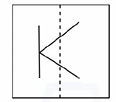
\includegraphics[width=0.5\columnwidth]{figs/2.png}
    \caption{}
    \label{fig:placeholder}
\end{figure}

\item A transparent square sheet shown above is folded along the dotted line. The folded sheet will look like
\begin{enumerate}
   
    \item 
        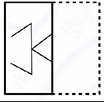
\includegraphics[width=0.25\columnwidth]{figs/2-a.png}
    
        \label{fig:placeholder}
    
        \item 
        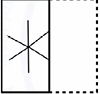
\includegraphics[width=0.25\columnwidth]{figs/2-b.png}
       
        \label{fig:placeholder}
   
        \item
        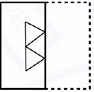
\includegraphics[width=0.25\columnwidth]{figs/2-c.png}
        
        \label{fig:placeholder}
    
\item 
        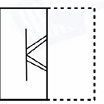
\includegraphics[width=0.25\columnwidth]{figs/2-d.png}
      
        \label{fig:placeholder}
  
      
\end{enumerate}


\item For a regular polygon having 10 sides, the interior angle between the sides of the polygon, in degrees, is:
\begin{enumerate}
    \begin{multicols}{2}
    \item 396
    \item 324
    \item 216
    \item 144
    \end{multicols}
\end{enumerate}


\item Which one of the following numbers is exactly divisible by 
\begin{align*}
(11^3+1)^2
\end{align*}

\begin{enumerate}
    \begin{multicols}{2}
    \item $11^2+1$
    \item $11^2+11$
    \item $11^2-1$
    \item $11^2-11$
    \end{multicols}
\end{enumerate}


\item \textit{Oasis is to sand as island is to \underline{\hspace{2cm}}} \\
Which one of the following options maintains a similar logical relation in the above sentence?
\begin{enumerate}
    \begin{multicols}{2}
    \item Stone
    \item Land
    \item Water
    \item Mountain
    \end{multicols}
\end{enumerate}



\item The importance of sleep is often overlooked by students when they are preparing for exams. Research has consistently shown that sleep deprivation greatly reduces the ability to focus on memory retention. Hence, cutting down on sleep to study longer hours can be counterproductive.  

Which one of the following statements is the CORRECT inference from the above passage?
\begin{enumerate}
    \begin{multicols}{2}
    \item Sleeping well alone is enough to prepare for an exam. Studying less number of hours is sufficient. 
    \item Students are efficient and not wrong in thinking that sleep is a waste of time. 
    \item If a student is extremely well prepared for an exam,he/she needn't sleep too much. 
    \item To do well in an exam, adequate sleep must be part of the preparation. 
    \end{multicols}
\end{enumerate}

\begin{figure}[H]
    \centering
    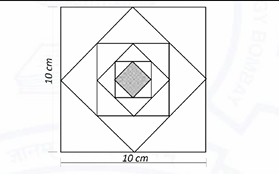
\includegraphics[width=0.5\columnwidth]{figs/7.png}
    \caption{}
    \label{fig:placeholder}
\end{figure}
\item In the figure shown above, each inside square is formed by joining the midpoints of the sides of the outer larger square. The area of the smallest square is $1 \,\text{cm}^2$. The area of the largest square is:
\begin{enumerate}
    \begin{multicols}{2}
    \item 12.50
    \item 6.25
    \item 3.125
    \item 1.5625
    \end{multicols}
\end{enumerate}



\item Let $X$ be a continuous random variable denoting the temperature measured.  
The range of temperature is $[0,100]$ degree Celsius and let the probability density function of $X$ be 
\begin{align*}
f(x) = 0.01 \quad \text{for } 0 \leq X \leq 100
\end{align*}  

The mean of $X$ is:
\begin{enumerate}
    \begin{multicols}{2}
    \item 5.0
    \item 25.0
    \item 50.0
    \item 2.5
    \end{multicols}
\end{enumerate}


\item The number of students passing or failing in an exam for a particular subject are presented in the bar chart.  
\begin{figure}[H]
    \centering
    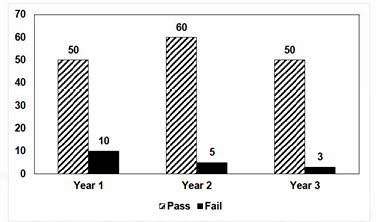
\includegraphics[width=0.5\columnwidth]{figs/9.png}
    \caption{}
    \label{fig:placeholder}
\end{figure}
Students who pass the exam cannot appear for the exam again. Students who fail the exam in the first attempt may appear for the exam in the following year. Students always pass the exam in their second attempt.  

The number of students who took the exam for the first time in the year 2 and year 3 respectively, are:
\begin{enumerate}
    \begin{multicols}{2}
    \item 65 and 53
    \item 60 and 50
    \item 55 and 50
    \item 55 and 48
    \end{multicols}
\end{enumerate}







\item Seven cars $P, Q, R, S, T, U$ and $V$ are parked in a row not necessarily in that order.  
The cars $T$ and $U$ should be parked next to each other.  
The cars $S$ and $V$ also should be parked next to each other, whereas $P$ and $Q$ cannot be parked next to each other.  
$Q$ and $S$ must be parked next to each other.  
$R$ is parked to the immediate right of $V$.  
$T$ is parked to the left of $U$.  

Based on the above statements, the only \textbf{INCORRECT} option given below is:

\begin{enumerate}
\item There are two cars parked in between $Q$ and $V$.
\item $Q$ and $R$ are not parked together.
\item $V$ is the only car parked in between $S$ and $R$.
\item Car $P$ is parked at the extreme end.
\end{enumerate}





\begin{center}
\Large \textbf{Electrical Engineering (EE)} \\[6pt]

\end{center}






\item Let $p$ and $q$ be real numbers such that \begin{align*}
    p^2+q^2=1
\end{align*}  
The eigenvalues of the matrix  
\[
\myvec{
p & q \\
q & -p
}
\]  
are

\begin{enumerate}
\begin{multicols}{2}
    

\item $i$ and $-i$
\item $1$ and $-1$
\item $pq$ and $-pq$
\item $pq$ and $-pq$
\end{multicols}
\end{enumerate}


\item Let 
\begin{align*}
p(z) &= z^3 + (2+i)z^2 + (2+3i)z + (i+2),
\end{align*}
where $z$ is a complex number. Which one of the following is true?

\begin{enumerate}
\item $\overline{p(z)} = p(\overline{z})$ for all $z$
\item The sum of the roots of $p(z)=0$ is a real number
\item The complex roots of the equation $p(z)=0$ occur in conjugate pairs
\item All the roots cannot be real
\end{enumerate}


\item Let $f(x)$ be a real-valued function such that $f''(x_0)=0$ for some $x_0 \in (0,1)$ and $f'''(x_0)\neq 0$ for all $x \in (0,1)$.  
Then $f(x)$ has

\begin{enumerate}
\item two local minima in $(0,1)$
\item one local minimum in $(0,1)$
\item exactly one local maximum in $(0,1)$
\item no distinct local minima in $(0,1)$
\end{enumerate}


\item For the network shown, the equivalent Thevenin voltage and Thevenin impedance as seen across terminals $a$-$b$ are:
\begin{figure}[H]
    \centering
    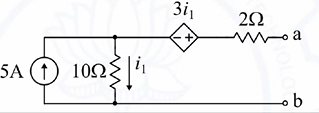
\includegraphics[width=0.5\columnwidth]{figs/14.png}
    \caption{}
    \label{fig:placeholder}
\end{figure}

\begin{enumerate}
\item $10 \angle 0^\degree$ V in series with $12\,\ohm$
\item $10 \angle 0^\degree$ V in series with $j2\,\ohm$
\item $5 \angle 0^\degree$ V in series with $j2\,\ohm$
\item $5 \angle 0^\degree$ V in series with $12\,\ohm$
\end{enumerate}


\item Which one of the following vector functions represents a magnetic field $\vec{B}(x,y,z)$, $x$, $y$, and $z$ are unit vectors along $x$-, $y$-, and $z$- axes, respectively?

\begin{enumerate}
\item $10x\hat{i}+20y\hat{j}-30z\hat{k}$
\item $10x\hat{i}+20y\hat{j}+10z\hat{k}$
\item $10x\hat{i}+20y\hat{j}-30z\hat{k}$
\item $10x\hat{i}-30x\hat{j}+20y\hat{z}$
\end{enumerate}










\item If the input $x(t)$ and output $y(t)$ of a system are related as  
\begin{align*}
    y(t) = \max(x(t),0),
\end{align*}
then the system is

\begin{enumerate}
\begin{multicols}{2}
    \item linear and time-variant
\item linear and time-invariant
\item non-linear and time-invariant
\item non-linear and time-variant
\end{multicols}
\end{enumerate}


\item Two discrete-time linear time-invariant systems with impulse responses  
\begin{align*}
    h_1[n] = ( \delta[n] + \delta[n-1] ), \quad h_2[n] = \delta[n] + \delta[n-2]
\end{align*}
are connected in cascade, where $\delta[n]$ is the Kronecker delta. The impulse response of the cascaded system is

\begin{enumerate}
\item $2\delta[n] + 2\delta[n-1] + \delta[n-2] + \delta[n-3]$
\item $\delta[n] + \delta[n-1] + 2\delta[n-2] + \delta[n-3]$
\item $\delta[n] + 2\delta[n-1] + \delta[n-2] + 2\delta[n-3]$
\item $\delta[n] + \delta[n-1] + \delta[n-2] + \delta[n-3]$
\end{enumerate}


\item Consider the table given:  

\begin{figure}[H]
    \centering
    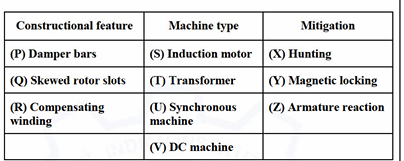
\includegraphics[width=0.5\columnwidth]{figs/8.png}
    \caption{}
    \label{fig:placeholder}
\end{figure}

The correct combination that relates the constructional feature, machine type and mitigation is

\begin{enumerate}
\item P-U-X, Q-V-Y, R-W-Z
\item P-U-X, Q-V-Z, R-W-Z
\item P-U-X, Q-V-Z, R-W-T
\item P-U-X, Q-V-T, R-W-Z
\end{enumerate}

\item Consider a power system consisting of $N$ number of buses. Buses in this system are categorized as generator (PV), load (PQ), and slack (O). The number of generator buses is $N_g$, the number of load buses is $N_l$. The balanced Newton-Raphson method is employed to solve the power flow problem. Let $\Delta P$, $\Delta Q$ and $\Delta |V|$ denote the mismatches. The Jacobian matrix $J$ is of the form below:

\[
\myvec{
\Delta P \\ \Delta Q
}
=
J \myvec{
\Delta \delta \\ \Delta |V|
}
\]

The dimension of the sub-matrix $J_1$ is

\begin{enumerate}
\begin{multicols}{2}
    \item $(N_g+N_l-1) \times (N_g+N_l-1)$
\item $(N_g+N_l-1) \times N_l$
\item $N_l \times (N_g+N_l-1)$
\item $N_l \times N_l$
\end{multicols}
\end{enumerate}


\item Two generators have cost functions in  h. Their incremental-cost characteristics are  

\begin{align*}
\frac{dF_1}{dP_1} &= 40 + 0.2 P_1, \\
\frac{dF_2}{dP_2} &= 30 + 0.4 P_2.
\end{align*}

They need to deliver a combined load of 260 MW. Ignoring the network losses, for economic operation, the generations $P_1$ and $P_2$ (in MW) are

\begin{enumerate}
\item $P_1 = 40, \, P_2 = 130$
\item $P_1 = 180, \, P_2 = 80$
\item $P_1 = 120, \, P_2 = 140$
\item $P_1 = 100, \, P_2 = 120$
\end{enumerate}

% Q11
\item For the closed-loop system shown, the transfer function is  

\begin{align*}
    \frac{C(s)}{R(s)} = \frac{E(s)}{R(s)} \cdot \frac{G}{1+GH}
\end{align*}

\begin{figure}[H]
    \centering
    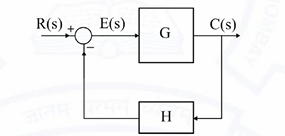
\includegraphics[width=0.5\columnwidth]{21.png}
    \caption{}
    \label{fig:placeholder}
\end{figure}
\begin{enumerate}
\begin{multicols}{2}
    \item $\dfrac{G}{1+GH}$ \\
\item $\dfrac{GH}{1+GH}$
\item $\dfrac{G}{1-GH}$ \\
\item $\dfrac{G}{1+G-H}$
\end{multicols}
\end{enumerate}






\item Inductance is measured by
\begin{enumerate}
    \begin{multicols}{2}
    \item Schering bridge
    \item Maxwell bridge
    \item Kelvin bridge
    \item Wien bridge
    \end{multicols}
\end{enumerate}

\item Suppose the circles 
\begin{align*}
    x^2 + y^2 + ax + 6 = 0
\end{align*}and 
\begin{align*}
    x^2 + y^2 + bx - 4 = 0
\end{align*}
intersect each other orthogonally at the point $(1,2)$.  
Then $a+b = \underline{\hspace{2cm}}$.


\item In the given circuit, the value of capacitor $C$ that makes current $i=0$ is
\begin{figure}[H]
    \centering
    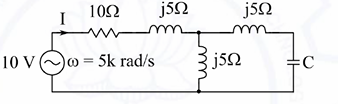
\includegraphics[width=0.5\columnwidth]{figs/24.png}
    \caption{}
    \label{fig:placeholder}
\end{figure}


\item Two single-core power cables have solid circular conductors of radius $0.7$ cm and are concentric with sheath.  
Both cables use the same dielectric of relative permittivity $2.5$.  
The capacitance of one cable is $80$ pF/m and the other is $100$ pF/m.  
The ratio of the dielectric thicknesses of the two cables is \underline{\hspace{2cm}}.


\item In the given circuit, for voltage $V = 10 \sin(\omega t)$ V, the value of $R$ should be 
\begin{figure}[H]
    \centering
    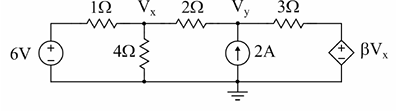
\includegraphics[width=0.5\columnwidth]{figs/26.png}
    \caption{}
    \label{fig:placeholder}
\end{figure}

\item A $1 \,\mu C$ point charge is held at the origin of a Cartesian coordinate system.  
A second point charge of $-1\,\mu C$ is moved from
$(0,10,0)$ m to $(5,5,5)$ and subsequently to $(5,0,0)$ then total work done is mJ.  




\item The power input to a $500\,$ V, $50\,$ Hz, 6-pole, 3-phase induction motor running at $975\,$ rpm is $60$ kW.  
The rotor copper loss is $1\,$ kW.  
If the total friction and windage losses are $2.5\,$ kW, then the efficiency is \underline{\hspace{2cm}} \%.


\item An alternator with internal voltage of $1\,$ pu and synchronous reactance of $0.4$ pu is connected by a transmission line to an infinite bus of $1\,$ pu voltage.  
The transmission line reactance is $0.1$ pu.  
The maximum power (in pu) that can be supplied by the alternator is \underline{\hspace{2cm}}.


\item The Bode magnitude plot for the transfer function $\dfrac{V_0(s)}{V_i(s)}$ of the circuit is shown.  
The value of $R$ is \underline{\hspace{2cm}} (round off to 2 decimal places).
\begin{figure}[H]
    \centering
    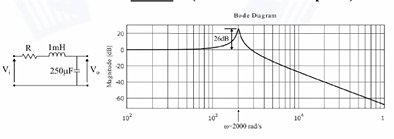
\includegraphics[width=0.5\columnwidth]{30.png}
    \caption{}
    \label{fig:placeholder}
\end{figure}




\item A signal generator having a source resistance of $50 \, \ohm$ is used to generate a $1$ kHz sinusoidal voltage.  
The open-circuit output voltage is $1$ V (rms). When connected to a load resistance $R_L = 50 \, \ohm$,  
the power delivered to the load (in mW, correct to one decimal place) is:  

\begin{enumerate}
\begin{multicols}{4}
    

\item 5.0
\item 7.1
\item 10.0
\item 20.0
\end{multicols}
\end{enumerate}


\item A $10$-bit successive binary up-counter is clocked with a frequency $f_{clk} = 100$ MHz.  
The maximum frequency that can be detected at the output of the most significant bit (MSB) Q9 is (in MHz):

\begin{enumerate}
\begin{multicols}{4}
    

\item 48.8
\item 50.0
\item 55.0
\item 55.6
\end{multicols}
\end{enumerate}

    \item In the circuit shown, the input $V_i$ is a sinusoidal AC voltage 
    having an RMS value of $230~\text{V} \pm 20\%$. 
    \begin{figure}[H]
        \centering
        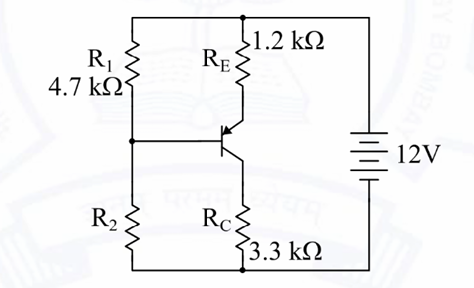
\includegraphics[width=0.5\columnwidth]{figs/33.png}
        \caption{}
        \label{fig:placeholder}
    \end{figure}
    The worst-case peak-inverse voltage (PIV) seen across any diode is 
     V. (Round off to 2 decimal places).

    \begin{multicols}{2}
    \begin{enumerate}
        \item 276.00 V
        \item 325.27 V
        \item 390.71 V
        \item 460.00 V
    \end{enumerate}
    \end{multicols}




\item In the BJT circuit shown, the $\beta$ of the PNP transistor is $100$.  
Assume $V_{BE} = 0.7$ V. The biasing resistors $R_1, R_2$ will be (in k$\ohm$):

\begin{figure}[H]
    \centering
    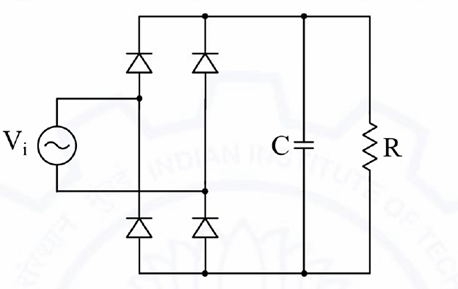
\includegraphics[width=0.5\columnwidth]{figs/34.png}
    \caption{}
    \label{fig:placeholder}
\end{figure}
\begin{enumerate}
\begin{multicols}{2}
    

\item $R_1 = 4.7$, $R_2 = 3.3$
\item $R_1 = 47$, $R_2 = 33$
\item $R_1 = 470$, $R_2 = 330$
\item $R_1 = 3.12$, $R_2 = 1.2$
\end{multicols}
\end{enumerate}


\item In the circuit shown, the input is a sinusoidal AC voltage having an RMS value of $230 \, V$ at $50$ Hz.  
The power dissipated across the resistor $R$ using two ideal diodes is (rounded off to 2 decimal places):

\begin{figure}[H]
    \centering
    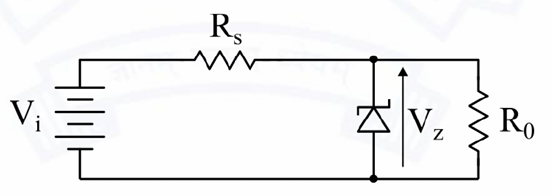
\includegraphics[width=0.5\columnwidth]{figs/35.png}
    \caption{}
    \label{fig:placeholder}
\end{figure}

\begin{enumerate}
\begin{multicols}{4}
    

\item 48.3 W
\item 50.2 W
\item 52.3 W
\item 55.0 W
\end{multicols}
\end{enumerate}


\item In the circuit shown, a $5$ V Zener diode is used to regulate the voltage across load $R_L$.  
The input is an unregulated DC voltage with minimum value of $8$ V and maximum value of $10$ V.  
The Zener diode has a maximum power dissipation of $2$ W. Ignoring the Zener diode's knee current,  
the minimum value of $R_s$ (in $\ohm$) is:

\begin{enumerate}
\begin{multicols}{4}
    

\item 8
\item 10
\item 12
\item 15
\end{multicols}
\end{enumerate}


\item Suppose the probability that a rain storm occurs in a town on any day is $p$, where $0 < p < 1$.  
If a rain storm occurs, it is independent of whether it has rained on earlier days.  
The probability that it rains on exactly the 5th day after no rain on the first 4 days is:

\begin{enumerate}
\begin{multicols}{4}
    

\item $(1-p)^4 p$
\item $(1-p)^5$
\item $p^5$
\item $\dfrac{p}{1-p}$
\end{multicols}
\end{enumerate}


\item Let $(1+j), (1-j), (5+j), (5-j)$ be the vertices of a rectangle in the complex plane.  
Assuming the contour is traversed counter-clockwise direction,  
the value of the contour integral $\oint_C \dfrac{dz}{z}$ is:

\begin{enumerate}
\begin{multicols}{4}
\item $j \pi$
\item $-j \pi$
\item $2 \pi j$
\item 0
\end{multicols}
\end{enumerate}





\item In the circuit, switch 'S' is in the closed position for a very long time. 
If the switch is opened at time $t=0$, then $i(t)$ in amperes, for $t \geq 0$ is


\begin{figure}[H]
    \centering
    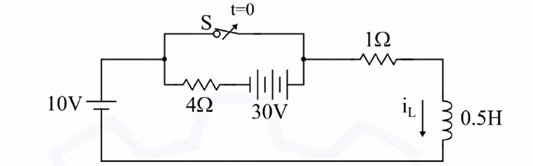
\includegraphics[width=0.5\columnwidth]{figs/39.png}
    \caption{}
    \label{fig:placeholder}
\end{figure}

\begin{multicols}{2}
\begin{enumerate}
    \item $8e^{-10t}$
    \item $10$
    \item $8+2e^{-10t}$
    \item $10(1-e^{-2t})$
\end{enumerate}
\end{multicols}


\item The input impedance, $Z_{in}(s)$, for the network shown is


\begin{figure}[H]
    \centering
    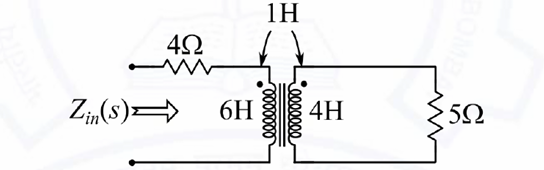
\includegraphics[width=0.5\columnwidth]{figs/40.png}
    \caption{}
    \label{fig:placeholder}
\end{figure}
\begin{multicols}{2}
\begin{enumerate}
    \item $6s+4$
    \item $7s+4$
    \item $\frac{2s^3+46s+20}{4s+5}$
    \item $\frac{2s^3+46s+20}{4s+5}$
\end{enumerate}
\end{multicols}

\item The causal signal with $z$-transform $\dfrac{z}{(z-a)^2}$ is  
($u[n]$ is the unit step signal)

\begin{multicols}{2}
\begin{enumerate}
    \item $a^n u[n]$
    \item $(n+1)a^n u[n]$
    \item $n a^{n-1}u[n]$
    \item $n^2 a^{n-2}u[n]$
\end{enumerate}
\end{multicols}


\item Let $f(t)$ be an even function, i.e. $f(-t) = f(t)$ for all $t$.  
Let the Fourier transform of $f(t)$ be defined as  
\begin{align*}
    F(\omega) = \int_{-\infty}^{\infty} f(t)e^{-j\omega t}dt
\end{align*}
Suppose  
\begin{align*}
    \frac{dF(\omega)}{d\omega} = -F(\omega)\quad \forall \, \omega,\quad F(0)=1
\end{align*}

\begin{multicols}{2}
\begin{enumerate}
    \item $F(\omega)=1$
    \item $F(\omega)=0$
    \item $F(\omega)=e^{-\omega}$
    \item $F(\omega)=e^{-\omega^2}$
\end{enumerate}
\end{multicols}

\item In a single-phase transformer, the total iron loss is $250$ W at nominal voltage of $440$ V and frequency $50$ Hz.  
The iron loss is $80$ W at $220$ V and $25$ Hz.  
Then, at nominal voltage and frequency, the hysteresis loss and eddy current loss respectively are

\begin{multicols}{2}
\begin{enumerate}
    \item 160 W and 90 W
    \item 200 W and 60 W
    \item 250 W and 200 W
    \item 50 W and 250 W
\end{enumerate}
\end{multicols}


\item In the figure shown, self-impedances of the two transmission lines are $j1.5\ \ohm$ each, and $j0.5\ \ohm$ is the mutual impedance.  
Both voltage sources in the figure are in phase. Given that $|E_1|=|E_2|=1$, the maximum steady-state real power that can be transferred from Bus-1 to Bus-2 is:
\begin{figure}[H]
    \centering
    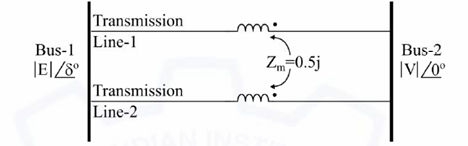
\includegraphics[width=0.5\columnwidth]{figs/44.png}
    \caption{}
    \label{fig:placeholder}
\end{figure}

\begin{multicols}{2}
\begin{enumerate}
    \item $|E_1|\,|E_2|$
    \item $\dfrac{|E_1|\,|E_2|}{2}$
    \item $2|E_1|\,|E_2|$
    \item $\dfrac{|E_1|\,|E_2|}{3}$
\end{enumerate}
\end{multicols}


\item A 3-Bus network is shown. Consider generators as ideal voltage sources. 
If rows 1, 2 and 3 of $Y_{bus}$ matrix correspond to Bus 1, 2 and 3 respectively, 
then $Y_{bus}$ of the network is

\begin{figure}[H]
    \centering
    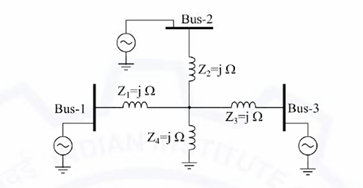
\includegraphics[width=0.5\columnwidth]{figs/45.png}
    \caption{}
    \label{fig:placeholder}
\end{figure}
\begin{multicols}{2}
\begin{enumerate}
\item $\myvec{
j4 & -j4 & 0 \\
-j4 & j6 & -j2 \\
0 & -j2 & j2
}$

\item $\myvec{
j2 & -j2 & 0 \\
-j2 & j6 & -j4 \\
0 & -j4 & j4
}$

\item $\myvec{
j4 & -j4 & 0 \\
-j4 & j8 & -j4 \\
0 & -j4 & j4
}$

\item $\myvec{
j2 & -j2 & 0 \\
-j2 & j4 & -j2 \\
0 & -j2 & j2
}$
\end{enumerate}
\end{multicols}


\item Suppose $I_a, I_b,$ and $I_c$ are a set of unbalanced current phasors in a three-phase system. 
The phase-B zero-sequence current = $I_{b0} = 0.1\angle 0^\degree$ p.u.  
Phase-A current, $I_a = 1\angle 0^\degree$ p.u. and phase-C current, $I_c = 0.2\angle 0^\degree$ p.u.  
Then $I_b$ in p.u. is 

\begin{multicols}{2}
\begin{enumerate}
\item $1.2 \angle 0^\degree$
\item $0.7 \angle 0^\degree$
\item $1 \angle -120^\degree + 0.1\angle 0^\degree$
\item $1 \angle -120^\degree - 0.1\angle 0^\degree$
\end{enumerate}
\end{multicols}

\item A counter is constructed with three D Flip-Flops. The logic output pairs are named $(Q_2,\overline{Q}_2), (Q_1,\overline{Q}_1), (Q_0,\overline{Q}_0)$. 
The counter is required to count the input clock pulses in the sequence as defined in the Gray-code: $000, 001, 011, 010, 110, 111, 101, 100$, repeatedly.  
Note that the bits are listed in $Q_2 Q_1 Q_0$ format.  
The combinational logic expression for input B is

\begin{multicols}{2}
\begin{enumerate}
\item $Q_0 Q_2$
\item $Q_0 Q_2 + Q_0 \overline{Q}_2$
\item $Q_0 \overline{Q}_1 + Q_2 \overline{Q}_1$
\item $Q_0 Q_1^n + Q_2 \overline{Q}_0$
\end{enumerate}
\end{multicols}


\item Let $A$ be a $10 \times 10$ matrix such that $A^T = -A$ is a null matrix, 
and let $I$ be the $10 \times 10$ identity matrix.  
The determinant of $A + I$ is  .


\item A three-phase balanced voltage is applied to the load shown. 
The phase sequence is RYB. The ratio $\dfrac{I_R}{I_Y}$ is

\begin{figure}[H]
    \centering
    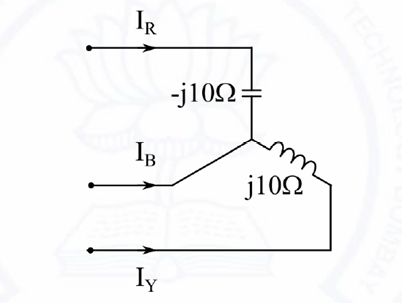
\includegraphics[width=0.5\columnwidth]{figs/49.png}
    \caption{}
    \label{fig:placeholder}
\end{figure}


\item In the given circuit, for maximum power to be delivered to $R_L$, its value should be  $\ohm$ (round off to 2 decimal places).

\begin{figure}[H]
    \centering
    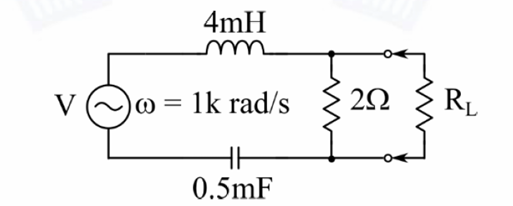
\includegraphics[width=0.5\columnwidth]{50.png}
    \caption{}
    \label{fig:placeholder}
\end{figure}




\item One coulomb of point charge moving with a uniform velocity $10 \, \hat{a}_x$ 
enters the region $z \geq 0$ having a magnetic flux density 
\begin{align*}
    \vec{B} = (10^{-3}y \, \hat{a}_x + 10^{-3}x \, \hat{a}_y) \, \text{T}.
\end{align*}
The magnitude of force on the charge at $t = 0^+$ is  N.  
($\hat{a}_x, \hat{a}_y, \hat{a}_z$ are unit vectors along x, y and z-axis respectively.)

\item Consider a large parallel plate capacitor. The gap $d$ between the two plates 
is filled entirely with a dielectric slab of relative permittivity $\epsilon_r$. 
The plates are initially charged to a potential difference of $V$ volts and are 
then disconnected from the source. If the dielectric slab is pulled out completely, 
the ratio of the new electric field $E_2$ in the gap to the original electric field 
$E_1$ is .

\item Consider a continuous-time signal $x(t)$ defined by $x(t) = 1$ for $|t| > 1$, 
and $x(t) = |t|$ for $|t| \leq 1$. Let the Fourier transform of $x(t)$ be defined as
\[
X(\omega) = \int_{-\infty}^{\infty} x(t) e^{-j\omega t} dt.
\]
The maximum magnitude of $X(\omega)$ is .

\item A belt-driven DC shunt generator running at 300 RPM delivers 100 kW to a 
200 V DC grid. It continues to run as a motor when the belt breaks, taking 10 kW 
from the DC grid. The armature resistance is $0.02~\Omega$, and the field resistance 
is $60~\Omega$. For the same field current in both operating conditions, the 
speed of the motor is  RPM. (Round off to 2 decimal places)

\item An 8-pole, 50 Hz, three-phase, slip-ring induction motor has an effective 
rotor resistance of 0.08 p.u. per phase. Its speed at maximum torque is 650 RPM. 
The additional resistance per phase that must be inserted in the rotor to achieve 
maximum torque at start is  $\Omega$. (Round off to 2 decimal places).  
Neglect magnetizing current and stator leakage impedance. Consider equivalent 
circuit parameters referred to stator.

\item Consider a closed-loop system as shown, 
\[
G_p(s) = \frac{144}{s(s+10)} \quad \text{is the plant transfer function, and} \quad 
G_c(s) = 1 \text{ is the compensator}.
\]  
\begin{figure}[H]
    \centering
    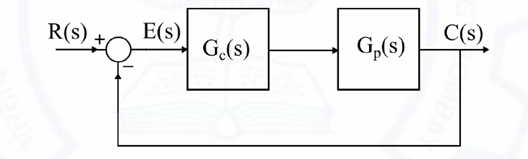
\includegraphics[width=0.5\columnwidth]{figs/56.png}
    \caption{}
    \label{fig:placeholder}
\end{figure}
For a unit-step input, the output response has damped oscillations. The damped 
natural frequency is  rad/s. (Round off to 2 decimal places)

\item In the given figure, plant $G_p(s) = \frac{2}{(s+10)(s+1)(s+2)}$ and 
compensator $G_c(s) = \frac{1+Ts}{1+T's}$. The external disturbance input is $D(s)$.  
It is desired that when the disturbance is a unit step, the steady-state error should 
not exceed 0.1 unit. The minimum value of $K$ is . (Round off to 1 decimal place)
\begin{figure}[H]
    \centering
    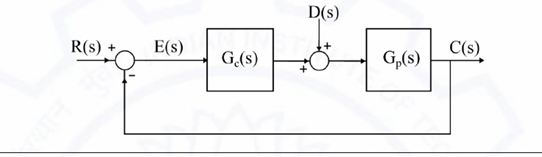
\includegraphics[width=0.5\columnwidth]{figs/57.png}
    \caption{}
    \label{fig:placeholder}
\end{figure}

\item The waveform shown in solid line is obtained by clipping a full-wave 
rectified sinusoid (shown dashed). The ratio of the RMS value of the full-wave 
rectified waveform to the RMS value of the clipped waveform is .  
(Round off to 2 decimal places)
\begin{figure}[H]
    \centering
    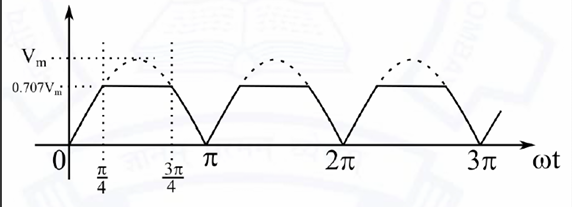
\includegraphics[width=0.5\columnwidth]{figs/58.png}
    \caption{}
    \label{fig:placeholder}
\end{figure}



\item The state space representation of a first-order system is given as
\[
\dot{x} = -x + u, \quad y = x
\]
where, $x$ is the state variable, $u$ is the control input and $y$ is the controlled output. Let $u = -Kx$, be the control law, where $K$ is the controller gain. To place a closed-loop pole at $-2$, the value of $K$ is

\begin{multicols}{2}
\begin{enumerate}
\item 1  
\item 2  
\item 3  
\item 4  
\end{enumerate}
\end{multicols}


\item An air-core radio frequency transformer as shown has a primary winding and a secondary winding. The mutual inductance $M$ between the windings of the transformer is \_ $\mu H$. (Round off to 2 decimal places).
\begin{figure}[H]
    \centering
    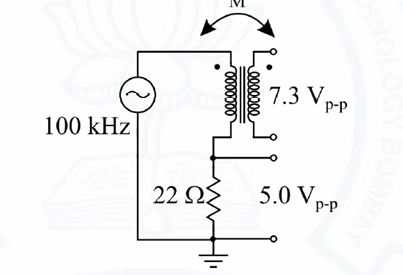
\includegraphics[width=0.5\columnwidth]{figs/60.png}
    \caption{}
    \label{fig:placeholder}
\end{figure}

\[
f = 100 \,\text{kHz}, \quad V_p = 22.05 \, V_{pp}, \quad V_s = 7.3 \, V_{pp}
\]


\item A 100 kHz square wave, switching between 0 V and 9 V, is applied to a CR high-pass filter circuit as shown. The resistance $R$ is 5 k$\Omega$ and the capacitance $C$ is 1 nF. The RMS output voltage of the circuit is \_ V. (Round off to 2 decimal places.)

\begin{figure}{H}
    \centering
    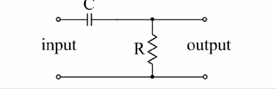
\includegraphics[width=0.5\columnwidth]{figs/61.png}
    \caption{}
    \label{fig:placeholder}
\end{figure}


\item A CMOS Schmitt-trigger inverter has a low output level of 0 V and a high output level of 5 V. Its input thresholds of 1.4 V and 2.4 V. The input capacitance and output resistance of the Schmitt-trigger are negligible. The frequency of the oscillator shown is \_ Hz. (Round off to 2 decimal places.)

\[
R = 10 \,\text{k}\Omega, \quad C = 47 \,\text{nF}
\]


\begin{figure}[H]
    \centering
    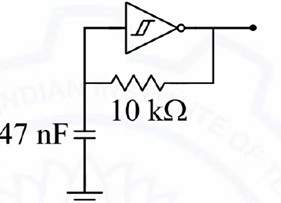
\includegraphics[width=0.5\columnwidth]{figs/62.png}
    \caption{}
    \label{fig:placeholder}
\end{figure}


\item Consider the boost converter shown. Switch Q is operating at 25 kHz with a duty cycle of 0.4. Assume the diode and switch to be ideal. Under steady-state condition, the average resistance $R_{eq}$ as seen by the source is \_ $\Omega$. (Round off to 2 decimal places.)

\[
V_{in} = 15 \, V, \quad L = 30 \,\mu H, \quad C = 100 \,\mu F, \quad R = 10 \,\ohm
\]


\begin{figure}[H]
    \centering
    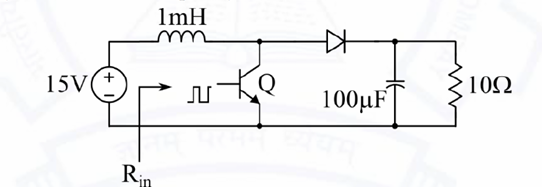
\includegraphics[width=0.5\columnwidth]{figs/63.png}
    \caption{}
    \label{fig:placeholder}
\end{figure}


\item Consider the buck-boost converter shown. Switch Q is operating at 25 kHz and 0.75 duty cycle. Assume diode and switch to be ideal. Under steady-state condition, the average current flowing into the inductor is \_ A. (Round off to 2 decimal places.)

\[
V_{in} = 20 \, V, \quad L = 1 \, mH, \quad C = 100 \,\mu F, \quad R = 10 \,\ohm
\]


\begin{figure}[H]
    \centering
    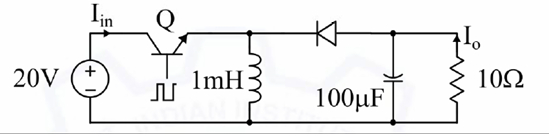
\includegraphics[width=0.5\columnwidth]{figs/64.png}
    \caption{}
    \label{fig:placeholder}
\end{figure}


\item A single-phase full-bridge inverter fed by a 325 V DC produces a symmetric quasi-square waveform across $ab$ as shown. To achieve a modulation index of 0.9, the angle $\phi$ expressed in degrees should be \_. (Round off to 2 decimal places.)

\[
V_{dc} = 325 \, V
\]


\textbf{}
\begin{figure}[H]
    \centering
    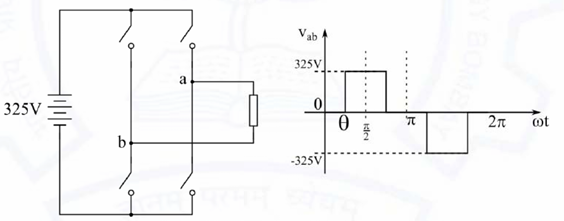
\includegraphics[width=0.5\columnwidth]{figs/65.png}
    \caption{}
    \label{fig:placeholder}
\end{figure}
\end{enumerate}



\end{flushleft}
\end{document}